\documentclass{standalone}

\usepackage{tikz}
\usepackage{graphics}

\begin{document}

\begin{tikzpicture}
\node (r) {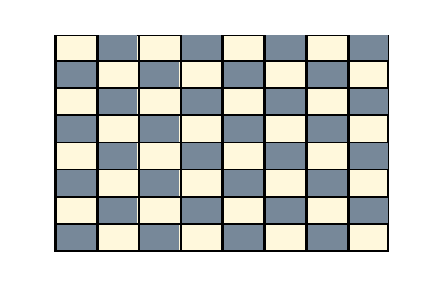
\includegraphics[scale=0.3]{raiz.png}};

\node (n1) [below of=r, yshift=-3cm] {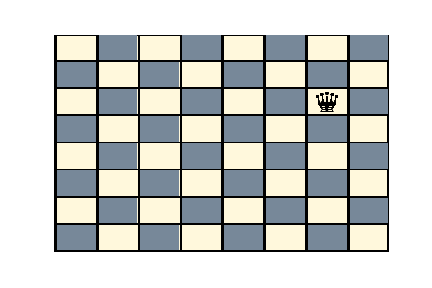
\includegraphics[scale=0.3]{n1.png}};     

\node (n2) [left of=n1, xshift=-4cm] {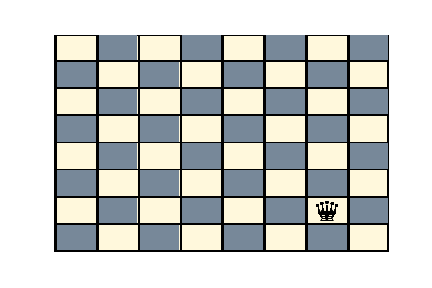
\includegraphics[scale=0.3]{n2.png}};     

\node (n3) [right of=n1, xshift=4cm] {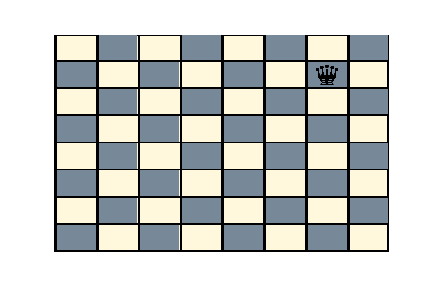
\includegraphics[scale=0.3]{n3.png}};

\node [right of=n3, xshift=2cm] {$\ldots$};

\draw[thick, ->] (r) -- (n1);

\draw[thick, ->] (r) -- (n2);

\draw[thick, ->] (r) -- (n3);

\end{tikzpicture}

\end{document}
